\section{独立随机变量与联合密度}
\label{sec:12-Real-Analysis-Support/06-Product-Measures-and-Fubini/03}

数据面板上常见这样一种做法：某一列画一张直方图，另一列再画一张，然后拿这两张图去推断两列同时取某个范围的比例。做法背后有一个没说出口的假设——联合分布等于两个边缘分布拼起来。上一节已经指出边缘记不住关联，这一节要问得更具体：什么时候可以把联合密度写成两个一元密度的乘积，以及写不成的时候，多出来的那部分长什么样。

\subsection{同样的边缘可以配上完全不同的联合}

先看一眼两幅图。它们的两条边缘密度曲线逐点相同，联合密度的等高线却是两副样子。

\begin{center}
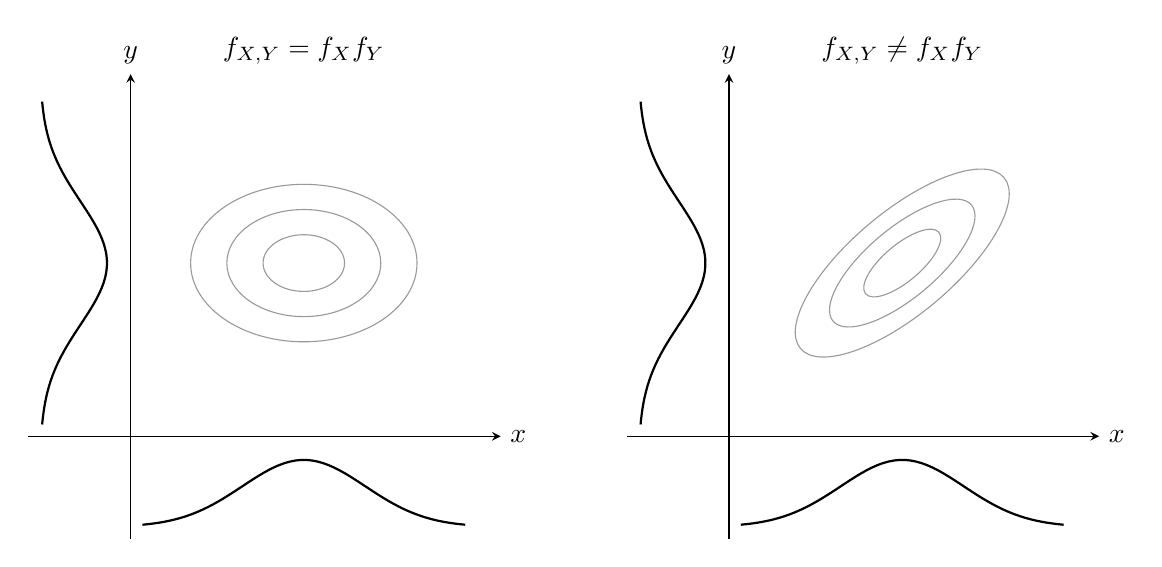
\begin{tikzpicture}[>=stealth]
% 左：可因式分解
\draw[->] (-1.3,0) -- (4.7,0) node[right] {\(x\)};
\draw[->] (0,-1.3) -- (0,4.6) node[above] {\(y\)};
\foreach \r in {0.45,0.85,1.25}
  \draw[gray!80] (2.2,2.2) ellipse ({1.15*\r} and {0.80*\r});
\draw[thick] plot[domain=0.15:4.25,samples=60]
  (\x,{-1.15+0.85*exp(-0.5*((\x-2.2)/0.78)^2)});
\draw[thick] plot[domain=0.15:4.25,samples=60]
  ({-1.15+0.85*exp(-0.5*((\x-2.2)/0.78)^2)},\x);
\node at (2.2,4.9) {\(f_{X,Y}=f_X f_Y\)};
% 右：不可因式分解
\begin{scope}[shift={(7.6,0)}]
\draw[->] (-1.3,0) -- (4.7,0) node[right] {\(x\)};
\draw[->] (0,-1.3) -- (0,4.6) node[above] {\(y\)};
\foreach \r in {0.45,0.85,1.25}
  \draw[gray!80,rotate around={40:(2.2,2.2)}] (2.2,2.2) ellipse ({1.35*\r} and {0.52*\r});
\draw[thick] plot[domain=0.15:4.25,samples=60]
  (\x,{-1.15+0.85*exp(-0.5*((\x-2.2)/0.78)^2)});
\draw[thick] plot[domain=0.15:4.25,samples=60]
  ({-1.15+0.85*exp(-0.5*((\x-2.2)/0.78)^2)},\x);
\node at (2.2,4.9) {\(f_{X,Y}\neq f_X f_Y\)};
\end{scope}
\end{tikzpicture}
\end{center}

\emph{两侧的边缘曲线完全一致；左边的等高线与坐标轴对齐，密度能拆成两个一元因子，右边倾斜的等高线拆不开。}

倾斜就是关联的形状。它在边缘上留不下痕迹——把二维密度分别沿两个方向压扁，两幅图给出同样的钟形曲线。

\subsection{因式分解与独立是同一件事}

设 \((X,Y)\) 相对于参考测度 \(\mu\times\nu\) 有联合密度 \(f_{X,Y}\)。这里的密度是 Radon--Nikodym 导数，参考测度可以是二维 Lebesgue 测度、两个计数测度的乘积，也可以是``计数测度乘 Lebesgue 测度''这种混合搭配——一个离散变量配一个连续变量同样适用。

\begin{proposition}
\(X\) 与 \(Y\) 独立，当且仅当存在只依赖 \(x\) 的非负可测函数 \(g\) 与只依赖 \(y\) 的非负可测函数 \(h\)，使得 \(f_{X,Y}(x,y)=g(x)h(y)\) 对 \(\mu\times\nu\) 几乎处处成立。
\end{proposition}

一个方向直接：独立意味着 \(P_{X,Y}=P_X\times P_Y\)，于是对任意可测矩形

\[
P(X\in A,\ Y\in B)
=\int_A f_X\,d\mu\int_B f_Y\,d\nu
=\int_{A\times B}f_X(x)f_Y(y)\,d(\mu\times\nu),
\]

中间那步把两个单积分并成一个二重积分，用的正是上一节的 Tonelli（被积函数非负，不必额外检查）。矩形构成 \(\pi\) 系并生成乘积 \(\sigma\)-代数，所以 \(f_Xf_Y\) 就是联合密度。

另一个方向要处理归一化。设 \(f_{X,Y}=gh\)。对 \(y\) 积分得边缘 \(f_X(x)=g(x)\int h\,d\nu\)，同理 \(f_Y(y)=h(y)\int g\,d\mu\)；再对全空间积分，得 \(\bigl(\int g\,d\mu\bigr)\bigl(\int h\,d\nu\bigr)=1\)。三式相乘一比对，\(f_X(x)f_Y(y)=g(x)h(y)=f_{X,Y}(x,y)\)。条件对账：两次交换积分次序都作用在非负函数上，Tonelli 无条件许可；结论只在几乎处处的意义下成立，因为密度本身只在几乎处处的意义下唯一。

命题的实用价值在于它把``检验独立''变成``盯着表达式看有没有耦合''。二元 Gaussian 密度里指数含 \(-\tfrac12(ax^2+2bxy+cy^2)\)，只要交叉项系数 \(b\neq0\)，指数就拆不成两半，图中右侧那种倾斜的等高线随之出现。\hyperref[sec:05-Probability/05-Joint-Distributions/02]{``随机变量的独立与依赖''}一篇用的是同一条判据，只是没有把参考测度和几乎处处写出来。

\subsection{独立让和的分布退化成卷积}

独立还有一个立刻可用的后果。设 \(X\perp Y\) 都有 Lebesgue 密度，\(Z=X+Y\)。用联合密度相乘写出分布函数，再交换积分次序，

\[
P(Z\le z)=\int\!\left(\int_{-\infty}^{z-x}f_Y(y)\,dy\right)f_X(x)\,dx ,
\]

对 \(z\) 求导得到

\[
f_Z(z)=\int_{-\infty}^{\infty}f_X(x)\,f_Y(z-x)\,dx=(f_X*f_Y)(z).
\]

换序一步靠 Tonelli，求导穿过积分号一步另需控制差商，条件见\hyperref[sec:12-Real-Analysis-Support/04-Limits-and-Integration/03]{``求导穿过积分号需要控制差商''}。两个独立 \(\Uniform(0,1)\) 的和给出在 \(z=1\) 处取峰的三角密度：和落在中间，可以由许多组 \((x,z-x)\) 实现，落在端点却只有一种方式。独立同分布样本的均值是 \(n\) 重卷积再缩放，形状一次比一次更接近钟形，这也是中心极限定理的几何侧影。更多算例见\hyperref[sec:05-Probability/05-Joint-Distributions/03]{``随机变量之和与卷积''}。

关键是卷积公式只对独立情形成立。相关变量的和不由两个边缘密度决定：图中左右两个联合分布的边缘完全一样，但 \(X+Y\) 的分布一个方差小、一个方差大，差别全部来自那项协方差。

\subsection{协方差为零只检查了一个函数}

把 \(X\) 取在 \(\set{-1,0,1}\) 上均匀，令 \(Y=X^2\)。此时 \(\E[X]=0\)，\(\E[XY]=\E[X^3]=0\)，于是 \(\Cov(X,Y)=0\)。但 \(Y\) 被 \(X\) 完全决定：\(P(X=1,Y=1)=1/3\)，而 \(P(X=1)P(Y=1)=(1/3)(2/3)=2/9\)。联合测度不等于乘积测度，全部质量压在抛物线上的三个点。

差距在于检查的范围。协方差为零只说 \(\E[g(X)h(Y)]=\E[g(X)]\E[h(Y)]\) 对 \(g(x)=x,\ h(y)=y\) 这一对成立；独立要求它对所有有界可测函数对都成立。一次等式与一整族等式，强度相差很远。联合 Gaussian 是常被引用的例外：它的密度由协方差矩阵完全决定，协方差为零直接抹掉交叉项，因式分解自动出现。这个便利不能推广到别的分布族——特征工程里两列相关系数接近零，并不构成``它们互不影响''的证据。

密度语言把独立性讲得很具体，代价是要求密度存在。没有密度的分布——落在低维子流形上的联合分布、混合了原子与连续部分的分布——依然可以用乘积测度定义独立，因式分解则要退回到测度的层面去写。生成模型里的隐变量常常正是这种情形，判断独立时不宜默认密度已经在手。
